\documentclass{standalone}
\usepackage{tikz}
\usetikzlibrary{decorations, decorations.text}
\usepackage{calc}
\usepackage{xcolor}
\usepackage{fontspec}
\newcommand{\cevapic}[1]{~{\fontspec{[ceva-c2.ttf]}#1}}
\definecolor{eins}{HTML}{e7e7e8}   %% Ring 1 "core"     - weiß - Mittelpunkt, Ring um Mittelpunkt
\definecolor{zwei}{HTML}{ed1c24}   %% Ring 2 "com"      - rot -  "Fenster" innen
\definecolor{drei}{HTML}{fbad18}   %% Ring 3  "culture" - orange - fünf Module, quasi invertiert
\definecolor{vier}{HTML}{74c043}   %% Ring 4  "creactiv" - grün -  vier Module
\definecolor{fuenf}{HTML}{0089d0}  %% Ring 5 "cience"  - cyan (blau) - drei Module mit "Strich"
\definecolor{sechs}{HTML}{11357e}  %% Ring 6 "carbon" -  indigo - viele "Fenster" außen
\definecolor{sieben}{HTML}{000000} %% Ring 7 "clamp" -  schwarz, c-förmig
\definecolor{cbase}{HTML}{222222}  %% Körper der Raumstation    
\begin{document}
 
% \tikzset{
%   pics/carc/.style args={#1:#2:#3:#4}{
%     code={
%       \draw[postaction={decorate, decoration={text along path, raise=-2pt, text align={align=center}, text={\cevapic{#4}}, reverse path}}] (#1:#3) arc(#1:#2:#3);
%     }
%   }
% }%
    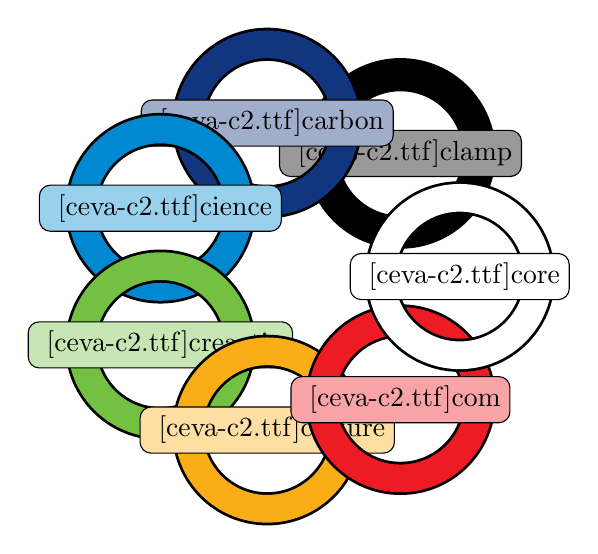
\begin{tikzpicture}[scale=0.4]
        % \draw[gray, line width=50pt] (0:0) circle (3);
        \foreach [count=\i] \ring/\color in
            {clamp/sieben,carbon/sechs,cience/fuenf,creactiv/vier,culture/drei,com/zwei,core/white}
            {%
                \draw[line width=12pt,draw=black] (\i*51.4286:5) circle (2.5);
                \draw[line width=10pt,draw=\color] (\i*51.4286:5) circle (2.5);
                \node [fill=\color!40,rounded corners,draw] at (\i*51.4286:5){\cevapic{\ring}};
                % \draw[color=\color!50,line width=45pt] (0:0) pic{carc=\i*51.418-25:\i*51.418+25:3:\ring};
            }%
            % \draw[color=white,line width=122] (0:0) pic{carc=-21:21:2.5:};
    \end{tikzpicture}
\end{document}
